
% Lecture Template for ME3001-001-Tristan Hill - Spring 2017 - Fall 2017 - Fall 2020 - Fall 2021
% Mechanical Engineering Analysis with MATLAB
% Module 1 - Introduction 
% Topic 2 - MATLAB Overview

% Document settings

\documentclass[handout]{beamer}  % for handout ?
\usepackage{/home/thill/Documents/lectures/analysis_lectures/analysis_lectures}

\newcommand{\MNUM}{1\hspace{2mm}} % Module number
\newcommand{\TNUM}{2\hspace{2mm}} % Topic number 
\newcommand{\moduletitle}{Introduction and MATLAB Review} % Titles and Stuff
\newcommand{\topictitle}{MATLAB Overview} 

\newcommand{\sectiontitleI}{What is MATLAB?} % More Titles and Stuff
\newcommand{\sectiontitleII}{Why use it? Why Not?}
\newcommand{\sectiontitleIII}{Review Basic Use}
\newcommand{\sectiontitleIV}{Hello World}

\newcommand{\btVFill}{\vskip0pt plus 1filll}

% custom box
\newsavebox{\mybox}

\author{ME3001 - Mechanical Engineering Analysis}  
\title{Lecture Module - \moduletitle}
\date{Mechanical Engineering\vspc Tennessee Technological University}

\begin{document}
	
	\lstset{language=MATLAB,basicstyle=\ttfamily\small,showstringspaces=false}
	
	\frame{\titlepage \center\begin{framed}\Large \textbf{Topic \TNUM - \topictitle}\end{framed} \vspace{5mm}}
	
	% Section 0: Outline
	\frame{
		\large \textbf{Topic \TNUM - \topictitle} \vspace{3mm}\\
		
		\begin{itemize}
			
			\item \sectiontitleI    \vspc % Section I
			\item \sectiontitleII 	\vspc % Section II
			\item \sectiontitleIII 	\vspc %Section III
			\item \sectiontitleIV 	\vspc %Section IV
			
		\end{itemize}
		
	}


\section{\sectiontitleI}

\frame{
  \frametitle{\sectiontitleI}
  			
  	\begin{itemize}
			\item High Level programming language
				\begin{itemize}
					\item language written in C++
					\item Interactive Development Environment written in JAVA 
					\item Windows, Mac, and Linux compatible
				\end{itemize}
			\item {\it MAT}rix {\it LAB}oratory
			\item {\it Technical Computing Language} - Mathworks
		\end{itemize}	

}

\section{\sectiontitleII}

\frame{ \small
  \frametitle{\sectiontitleII}
  
  \begin{itemize}
			\item A powerful tool for engineers, scientists, and students
				\begin{itemize}	
					\item  optimized for floating point arithmetic and linear algebra
					\item extensive library of mathematical functions and operations 
					\item specialized functions and operations
						\begin{itemize}
							\begin{multicols}{2}
							\item Aerospace
							\item Robotics
							\item Communications
							\item Image/Signal Processing 
							\item Embedded Systems and Controls
							\end{multicols}
						\end{itemize}
					\item ability to use {\it symbolic programming }	
				\end{itemize}
			\item Ease of Access and Community
				\begin{itemize}
					\item {\it Plug and Play}, it works out of the box
					\item requires no programming experience to begin
					\item online community for sharing code,  {\it MATLAB Central}
				\end{itemize}
		\end{itemize}

}
\section{\sectiontitleIII}

\frame{
  \frametitle{\sectiontitleIII}
	
\textbf{Useful Commands( type in Command Window)} \vspace{3mm}\\

		
			\scalebox{1.25}{{\fontfamily{qcr}\selectfont  \hspace{5mm} >>  clear variables}} \vspace{3mm}\\
			\scalebox{1.25}{{\fontfamily{qcr}\selectfont  \hspace{5mm} >>  clc}} \vspace{3mm}\\
			\scalebox{1.25}{{\fontfamily{qcr}\selectfont  \hspace{5mm} >>  close all}} \vspace{3mm}\\
			\scalebox{1.25}{{\fontfamily{qcr}\selectfont  \hspace{5mm} >>  }} \\

	
}	
\frame{
  \frametitle{\sectiontitleIII}
	
		
		
				\textbf{ Common Mathematics Functions} \vspace{3mm}\\	
					\begin{itemize}
						\item \scalebox{1.25}{{\fontfamily{qcr}\selectfont  \hspace{5mm} sqrt()}} \vspace{3mm}\\
						\item \scalebox{1.25}{{\fontfamily{qcr}\selectfont  \hspace{5mm} exp()}} \vspace{3mm}\\
						\item \scalebox{1.25}{{\fontfamily{qcr}\selectfont  \hspace{5mm} log()}} \vspace{3mm}\\
						\item \scalebox{1.25}{{\fontfamily{qcr}\selectfont  \hspace{5mm} log2()}} \vspace{3mm}\\
						\item \scalebox{1.25}{{\fontfamily{qcr}\selectfont  \hspace{5mm} log10()}} \\
					\end{itemize}	

}

\frame{
  \frametitle{\sectiontitleIII}
	

		
		
			\textbf{ Other Useful Functions} \\	
					\begin{multicols}{2}	
					\begin{itemize}
						\item \scalebox{1.0}{{\fontfamily{qcr}\selectfont  \hspace{5mm} round()}} \\
						\item \scalebox{1.0}{{\fontfamily{qcr}\selectfont  \hspace{5mm} floor()}} \\
						\item \scalebox{1.0}{{\fontfamily{qcr}\selectfont  \hspace{5mm} int8()}} \\
						\item \scalebox{1.0}{{\fontfamily{qcr}\selectfont  \hspace{5mm} sign()}} \\
						\item \scalebox{1.0}{{\fontfamily{qcr}\selectfont  \hspace{5mm} mod()}} \\
						\item \scalebox{1.0}{{\fontfamily{qcr}\selectfont  \hspace{5mm} rem()}} \\
						\item \scalebox{1.0}{{\fontfamily{qcr}\selectfont  \hspace{5mm} fzero()}} \\
					\end{itemize}	
					\end{multicols}
					
				\textbf{ Built-in Constants} \\		
					\begin{multicols}{2}
						\begin{itemize}
					
					\item \scalebox{1.0}{{\fontfamily{qcr}\selectfont  \hspace{5mm} pi}} \vspace{1mm}\\
					\item \scalebox{1.0}{{\fontfamily{qcr}\selectfont  \hspace{5mm} i}} \vspace{1mm}\\
					\item \scalebox{1.0}{{\fontfamily{qcr}\selectfont  \hspace{5mm} j}} \vspace{1mm}\\
					\item \scalebox{1.0}{{\fontfamily{qcr}\selectfont  \hspace{5mm} inf}} \vspace{1mm}\\
					\item \scalebox{1.0}{{\fontfamily{qcr}\selectfont  \hspace{5mm} NaN}} \vspace{1mm}\\

				\end{itemize}
				\end{multicols}
}



\frame{
  \frametitle{\sectiontitleIII}
	
\textbf{The Built in Help } \vspace{3mm}\\
\begin{itemize}	
					\item 	\scalebox{1.0}{{\fontfamily{qcr}\selectfont  \hspace{5mm} >> help fzero()}} \vspace{3mm}\\
						\item use the help to get information about the built in functions  \vspace{3mm}\\
						\item the full documentation is also available online  \vspace{3mm}\\
				\end{itemize}		
						
						 

}
						
					
\section{\sectiontitleIV}

\frame{
  \frametitle{\sectiontitleIV}
  
This is the classic first exercise for any programming language. \vspace{10mm}\\

	\scalebox{1.0}{{\fontfamily{qcr}\selectfont  \hspace{5mm} >> Hello World}} \vspace{3mm}\\

}

\end{document}

		

%	\item \textbf{ \LARGE Main Topics to be Covered}\\
%	\Large{ Mathematical Modeling of Engineering Problems Involving: }\\
%		\begin{enumerate}
%			\item Solutions to Non-Linear Equations \vspace{5mm}\\
%				\begin{itemize}
%					\item Rigid Body Dynamics \\
%					
%					\item Optimization and Design \\
%					
%				\end{itemize}
%			
%			\item Solving Systems Linear Equations \vspace{5mm}\\
%				\begin{multicols}{2}
%				\begin{itemize}
%					\item Statics and Structural  \\
%					
%					\item Equilibrium Equations\\
%					
%					\item The Eigenvalue Problem\\
%					
%					\item Mechanisms and Machines\\
%					
%				\end{itemize}
%				\end{multicols}
%			\item Ordinary Differential Equations \vspace{5mm}\\
%				\begin{multicols}{2}
%				\begin{itemize}
%					\item Rigid Body Dynamics\\
%					\item Thermodynamics and Heat Transfer\\
%					\item Electronics and Circuits\\
%				\end{itemize}
%				\end{multicols}
%			\item Partial Differential Equations \vspace{5mm}\\
%				\begin{itemize}
%					\item Fluid Dynamics\\
%					\item Thermodynamics and Heat Transfer\\
%				\end{itemize}
%		\end{enumerate}
%	\end{itemize}
%	\LARGE
%	\begin{enumerate}	
%		
%		\item \textbf{  Solutions to Non-Linear Equations}\\
%			\begin{itemize}
%					\item What is a non-linear equation? \vspace{20mm} \\
%					\item What does it mean to solve a non-linear equation? \vspace{20mm} \\
%					\item Standard form of this problem:\\
%					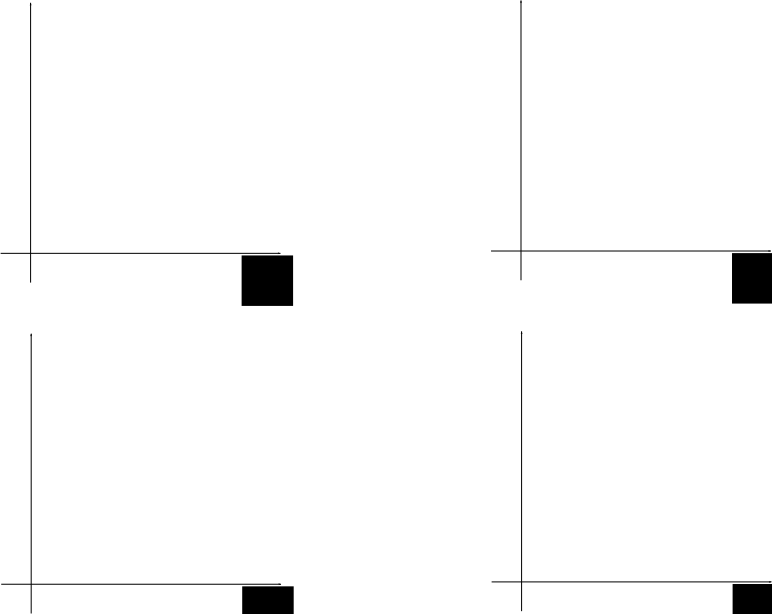
\includegraphics[scale=.5]{lecture1_fig1.png}
%			\end{itemize}
%\newpage			
%			\item \textbf{  Solving Systems Linear Equations}\\
%			\begin{itemize}
%					\item What is a system of linear equations?\vspace{20mm} \\
%					\item What does it mean to solve a  system of linear equations? \vspace{20mm} \\
%					\item A very simple example:\\
%					\includegraphics[scale=.45]{lecture1_fig2.png}
%			\end{itemize}
%			
%			\item \textbf{  Ordinary Differential Equations}\\
%			\begin{itemize}
%					\item What is a Differential Equations? What about a system of them?\vspace{20mm} \\
%					\item What does it mean to solve a differential equation? \vspace{20mm} \\
%					\item A very simple example:\\
%					\includegraphics[scale=.6]{lecture1_fig3.png}\\
%					\Large {ODE:}\vspace{30mm}\\
%					\Large {Solution:}\\
%			\end{itemize}
%\newpage			
%			\item \textbf{  Partial Differential Equations}\\ 
%			\begin{itemize}
%					\item What is different about a Partial Differential Equation? \vspace{20mm} \\
%					
%					\item What is different about the solution to a PDE?  \vspace{20mm}  \\
%					
%					\item What does this allow us to do? \\
%					
%			\end{itemize}
%	\end{enumerate}
		



	





